\documentclass[../main.tex]{subfiles}

\begin{document}

\chapter*{PREFACE}
\label{cha:cha_P_1}
\addcontentsline{toc}{section}{PREFACE}

This book is designed to support a one-semester course in numerical methods. It has been
written for students who want to learn and apply numerical methods in order to solve problems in engineering and science. As such, the methods are motivated by problems rather
than by mathematics. That said, sufficient theory is provided so that students come away
with insight into the techniques and their shortcomings.


$\text{MATLAB}^\copyright$  provides a great environment for such a course. Although other environments (e.g., Excel/VBA, Mathcad) or languages (e.g., Fortran 90, C++) could have
been chosen, MATLAB presently offers a nice combination of handy programming features with powerful built-in numerical capabilities. On the one hand, its M-file programming environment allows students to implement moderately complicated algorithms in a
structured and coherent fashion. On the other hand, its built-in, numerical capabilities
empower students to solve more difficult problems without trying to "reinvent the wheel."


The basic content, organization, and pedagogy of the second edition are essentially
preserved in the third edition. In particular, the conversational writing style is intentionally
maintained in order to make the book easier to read. This book tries to speak directly to the
reader and is designed in part to be a tool for self-teaching.

That said, this edition differs from the past edition in three major ways: (1) two new
chapters, (2) several new sections, and (3) revised homework problems.
\begin{enumerate}
	\item  \textbf{New Chapters.} As shown in \ref{fig:fig_P_1}, I have developed two new chapters for this edition. Their inclusion was primarily motivated by my classroom experience. That is,
they are included because they work well in the undergraduate numerical methods
course I teach at Tufts. The students in that class typically represent all areas of engineering and range from sophomores to seniors with the majority at the junior level. In
addition, we typically draw a few math and science majors. The two new chapters are:
\begin{itemize}
	\item \textbf{Eigenvalues.} When I first developed this book, I considered that eigenvalues might
be deemed an "advanced" topic. I therefore presented the material on this topic at
the end of the semester and covered it in the book as an appendix. This sequencing
had the ancillary advantage that the subject could be partly motivated by the role of
eigenvalues in the solution of linear systems of ODEs. In recent years, I have begun




to move this material up to what I consider to be its more natural mathematical position at the end of the section on linear algebraic equations. By stressing applications (in particular, the use of eigenvalues to study vibrations), I have found that
students respond very positively to the subject in this position. In addition, it allows
me to return to the topic in subsequent chapters which serves to enhance the
students’ appreciation of the topic.
\item  \textbf{Fourier Analysis.} In past years, if time permitted, I also usually presented a lecture
at the end of the semester on Fourier analysis. Over the past two years, I have begun
presenting this material at its more natural position just after the topic of linear least
squares. I motivate the subject matter by using the linear least-squares approach to
fit sinusoids to data. Then, by stressing applications (again vibrations), I have found
that the students readily absorb the topic and appreciate its value in engineering and
science.


It should be noted that both chapters are written in a modular fashion and could
be skipped without detriment to the course's pedagogical arc. Therefore, if you
choose, you can either omit them from your course or perhaps move them to the
end of the semester. In any event, I would not have included them in the current
edition if they did not represent an enhancement within my current experience in
the classroom. In particular, based on my teaching evaluations, I find that the
stronger, more motivated students actually see these topics as highlights. This is
particularly true because MATLAB greatly facilitates their application and interpretation.
\end{itemize}
\item \textbf{New Content.} Beyond the new chapters, I have included new and enhanced sections on a
number of topics. The primary additions include sections on animation (Chap. 3), Brent's
method for root location (Chap. 6), \textsl{LU} factorization with pivoting (Chap. 8), \textsl{random numbers and Monte Carlo simulation} (Chap. 14), \textsl{ adaptive quadrature} (Chap. 20),and \textsl{event termination of ODEs} (Chap. 23).


\item \textbf{New Homework Problems.} Most of the end-of-chapter problems have been modified, and a variety of new problems have been added. In particular, an effort has been
made to include several new problems for each chapter that are more challenging and
difficult than the problems in the previous edition.
\end{enumerate}

\begin{figure}[H]
	\centering
	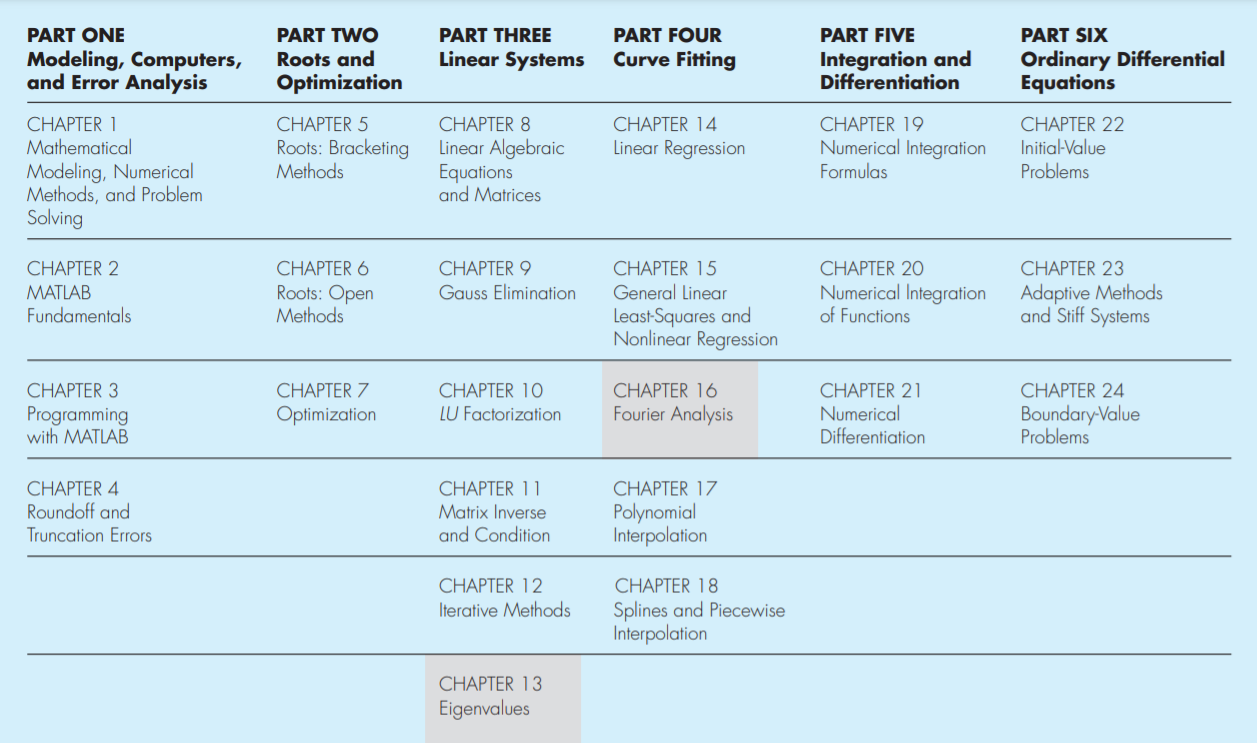
\includegraphics[width=1\linewidth]{fig_P_1.png}
	\caption{\textsf{An outline of this edition. The shaded areas represent new material. In addition, several of the original chapters have been supplemented with
new topics.}}
	\label{fig:fig_P_1}
\end{figure}


Aside from the new material and problems, the third edition is very similar to the second.
In particular, I have endeavored to maintain most of the features contributing to its pedagogical effectiveness including extensive use of worked examples and engineering and scientific applications. As with the previous edition, I have made a concerted effort to make this
book as "student-friendly" as possible. Thus, I’ve tried to keep my explanations straightforward and practical.
Although my primary intent is to empower students by providing them with a sound
introduction to numerical problem solving, I have the ancillary objective of making this
introduction exciting and pleasurable. I believe that motivated students who enjoy engineering and science, problem solving, mathemati cs and yes programming, will ultimately make better professionals. If my book fosters enthusiasm and appreciation for these
subjects, I will consider the effort a success.

\textbf{Acknowledgments}. Several members of the McGraw-Hill team have contributed to
this project. Special thanks are due to Lorraine Buczek, and Bill Stenquist, and Melissa
Leick for their encouragement, support, and direction. Ruma Khurana of MPS Limited, a
Macmillan Company also did an outstanding job in the book’s final production phase. Last,
but not least, Beatrice Sussman once again demonstrated why she is the best copyeditor in
the business.
During the course of this project, the folks at The MathWorks, Inc., have truly demonstrated their overall excellence as well as their strong commitment to engineering and
science education. In particular, Courtney Esposito and Naomi Fernandes of The MathWorks, Inc., Book Program have been especially helpful.
The generosity of the Berger family, and in particular Fred Berger, has provided me
with the opportunity to work on creative projects such as this book dealing with computing
and engineering. In addition, my colleagues in the School of Engineering at Tufts, notably
Masoud Sanayei, Lew Edgers, Vince Manno, Luis Dorfmann, Rob White, Linda Abriola,
and Laurie Baise, have been very supportive and helpful.
Significant suggestions were also given by a number of colleagues. In particular, Dave
Clough (University of Colorado–Boulder), and Mike Gustafson (Duke University) provided valuable ideas and suggestions. In addition, a number of reviewers provided useful
feedback and advice including Karen Dow Ambtman (University of Alberta), Jalal Behzadi
(Shahid Chamran University), Eric Cochran (Iowa State University), Frederic Gibou (University of California at Santa Barbara), Jane Grande-Allen (Rice University), Raphael
Haftka (University of Florida), Scott Hendricks (Virginia Tech University), Ming Huang
(University of San Diego), Oleg Igoshin (Rice University), David Jack (Baylor University), Clare McCabe (Vanderbilt University), Eckart Meiburg (University of California at
Santa Barbara), Luis Ricardez (University of Waterloo), James Rottman (University of
California, San Diego), Bingjing Su (University of Cincinnati), Chin-An Tan (Wayne State
University), Joseph Tipton (The University of Evansville), Marion W. Vance (Arizona
State University), Jonathan Vande Geest (University of Arizona), and Leah J. Walker
(Arkansas State University).
It should be stressed that although I received useful advice from the aforementioned
individuals, I am responsible for any inaccuracies or mistakes you may find in this book.
Please contact me via e-mail if you should detect any errors.
Finally, I want to thank my family, and in particular my wife, Cynthia, for the love,
patience, and support they have provided through the time I’ve spent on this project.
\newpage


\begin{flushright}
Steven C. Chapra\\
Tufts University



Medford, Massachusetts\\
steven.chapra@tufts.edu\\
\end{flushright}


\bigskip
\section*{PEDAGOGICAL TOOLS}
\label{sec:sec_P_1_1}


\textbf{Theory Presented as It Informs Key Concepts.} The text is intended for Numerical Methods users, not developers. Therefore, theory is not included for “theory’s sake,” for example no
proofs. Theory is included as it informs key concepts such as the Taylor series, convergence,
condition, etc. Hence, the student is shown how the theory connects with practical issues in
problem solving.


\textbf{Introductory MATLAB Material.} The text includes two introductory chapters on how to
use MATLAB. Chapter 2 shows students how to perform computations and create graphs
in MATLAB’s standard command mode. Chapter 3 provides a primer on developing
numerical programs via MATLAB M-file functions. Thus, the text provides students with
the means to develop their own numerical algorithms as well as to tap into MATLAB’s
powerful built-in routines.

\textbf{Algorithms Presented Using MATLAB M-files.} Instead of using pseudocode, this book
presents algorithms as well-structured MATLAB M-files. Aside from being useful computer programs, these provide students with models for their own M-files that they will
develop as homework exercises.

\textbf{Worked Examples and Case Studies.} Extensive worked examples are laid out in detail
so that students can clearly follow the steps in each numerical computation. The case studies consist of engineering and science applications which are more complex and richer than
the worked examples. They are placed at the ends of selected chapters with the intention of
(1) illustrating the nuances of the methods, and (2) showing more realistically how the
methods along with MATLAB are applied for problem solving.

\textbf{Problem Sets.} The text includes a wide variety of problems. Many are drawn from engineering and scientific disciplines. Others are used to illustrate numerical techniques and
theoretical concepts. Problems include those that can be solved with a pocket calculator as
well as others that require computer solution with MATLAB.

\textbf{Useful Appendices and Indexes.} Appendix A contains MATLAB commands, and
Appendix B contains M-file functions.

\textbf{Textbook Website.} A text-specific website is available at www.mhhe.com/chapra. Resources include the text images in PowerPoint, M-files, and additional MATLAB resources.
\blankpage

\end{document}